\documentclass[thesis.tex]{subfiles}
\newcommand\TPR{\mathit{TPR}}
\newcommand\FPR{\mathit{FPR}}
\newcommand\OMP{\mathit{1-P}}
\newcommand\TP{\mathit{TP}}
\newcommand\FP{\mathit{FP}}
\newcommand\TN{\mathit{TN}}
\newcommand\FN{\mathit{FN}}
\newcommand\ROC{ROC}
\newcommand\PR{PR}

\begin{document}
\chapter{Image correspondence}
\label{sec:ic}
%
In this chapter we explain the image correspondence problem and the application of our descriptor to solve it.

Image correspondence is the problem of matching features across two images $A$ and $B$ of the same object. A match should ideally indicate that the two features correspond to the same physical point or object. The two images of the object can be captured under different lighting conditions, taken from different positions, and have varying tilt, rotation, zoom, and focus; hence the images will differ based on these variables. By using an interest point detector in combination with a descriptor, we are able to find interest points in $A$ and $B$, describe each interest point with a descriptor algorithm, and compare these descriptors across the two images by a given similarity measure to estimate whether the points match.

The chapter is structured as follows. First we describe the steps of our approach: the strategy to select matches between images, the similarity measure used for this, and the the measure used to evaluate matching performance. We then describe the dataset and how to use it to determine correctness of matches, and specify our experimental setup. In order to visualize our approach, we then extend the earlier example with image correspondence. Finally, we present our parameter optimization and test results, which include a comparison with SIFT.
%
\section{Matching strategies}
\label{sec:matching_strategies}
%
The matching performance depends on the matching strategy. \citet{mikolajczyk2005performance} described the following three matching strategies that are used when solving the image correspondence problem:
Simple \emph{thresholding} compares each descriptor in image $A$ with each descriptor in image $B$. Any two descriptors having a mutual distance below a threshold $t$ are classified as matches (positive). \emph{Best-thresholding} finds the best matching descriptor in $B$ for each descriptor in $A$. If the distance is below a threshold $t$, it is a match (positive), and otherwise it is rejected (negative). \emph{Ratio-thresholding} finds the two best matching descriptors in $B$ with distances $B_1$ and $B_2$ for each descriptor in $A$. If the ratio between the two distances ($\frac{B_1}{B_2}$) to the descriptor in $A$ is below a threshold $t$, it is a match (positive). Otherwise the match is rejected (negative). In other words a distance ratio close to 0 is a good match.

We choose the ratio-thresholding strategy since this is the one favoured in previous image correspondence evaluations \cite{mikolajczyk2005performance,dahl2011finding,larsen2012jet,lowe2004distinctive}. Additionally this matching strategy is more general since it uses the ratio between the distance to the two best matching features instead of the absolute values giving less dependence on the descriptor in question. The two following cases give a good rationale for choosing this matching strategy: The first case is when two descriptors are good matches. In this case the descriptors will be very similar, and their difference could be caused by noise or other small variations. Due to this fact the algorithm shouldn't choose one over the other and hence the matching is negative since the distance ratio is close to 1. The second case is when only poorly matching descriptors are present. In this case the distance to both of the best matching descriptors will be high and the distance ratio close to 1 giving us a negative match as desired.


\section{Similarity measure}
\label{sec:similarity_measure}
We need a similarity measure in order to compute the distance between two descriptors. The Euclidean distance is widely used as similarity measure in the literature \cite{lowe2004distinctive,ke2004pca,mikolajczyk2005performance}. \citet{larsen2012in} evaluated the following different similarity measures: $L_1$ distance, Euclidean distance, $\chi^2$ distance, Kullback-Leibler divergence, and Jensen-Shannon divergence, and he found no notable difference in performance for his locally orderless-based descriptor. Based on this and some preliminary tests of our descriptor, where Euclidean distance ($L_2$) slightly outperformed $L_1$-distance, we choose to use Euclidean distance.

\section{Performance measures}
\label{sec:performance_measures}

Having established the matching strategy and similarity measure, we now describe the two performance measures which we use for evaluation of descriptor algorithms.

Assume that we have computed the descriptor distances, found the two best matching descriptors in $B$ for each descriptor in $A$ and computed their distance ratio $r$. We now wish to compute the performance of the descriptor algorithm utilized. The problem has been reduced to a binary classification problem of whether two descriptors match or not. Following the approach described in \Cref{sec:binaryClassificationMeasures}, using $r$ as the classification score $s$, we are able to compute the PR- and ROC-curves as well as their AUCs to get a measure of the performance of our descriptor.

Recall the discussion of the benefits of ROC and PR in \Cref{sec:binaryClassificationMeasures}. The PR measure is beneficial to use when the positive class is of greater importance than the negative class. In the image correspondence problem we wish to find as many corresponding points as possible and hence the PR measure has greater importance than the ROC measure. This however doesn't mean that it isn't important to be able to classify negatives.

%The approach is similar to that of \citet{winder2009picking,dahl2011finding}.

\section{Dataset}
\label{sec:dtuDataset}
The dataset we use for training and evaluation of our descriptor is called the \emph{DTU Robot 3D dataset} \cite{aanaes2010recall} (from now on called the DTU dataset). It consists of images of objects taken in a closed black box with varying illumination using 19 fixed position LED lights. In total there are 60 scenes with varying objects. \Cref{fig:dtu_examples} shows 4 example scenes. \citet{aanaes2010ground} classify the scenes into categories as shown in \Cref{tbl:dtu_scene_classifications}.

\begin{figure}[p]
	\centering
	\begin{subfigure}{0.49\textwidth}
		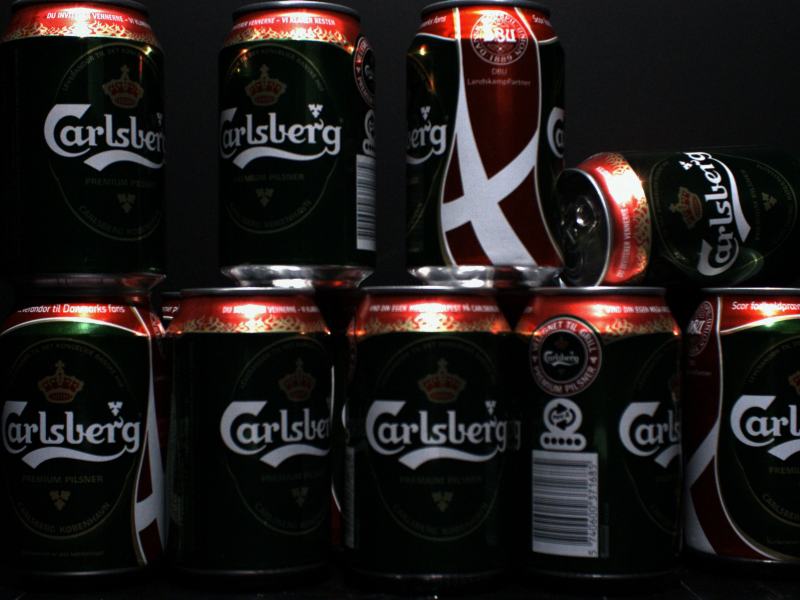
\includegraphics[width=\textwidth]{img/dtu_example_1.png}
	\end{subfigure}
	\hfill
	\begin{subfigure}{0.49\textwidth}
		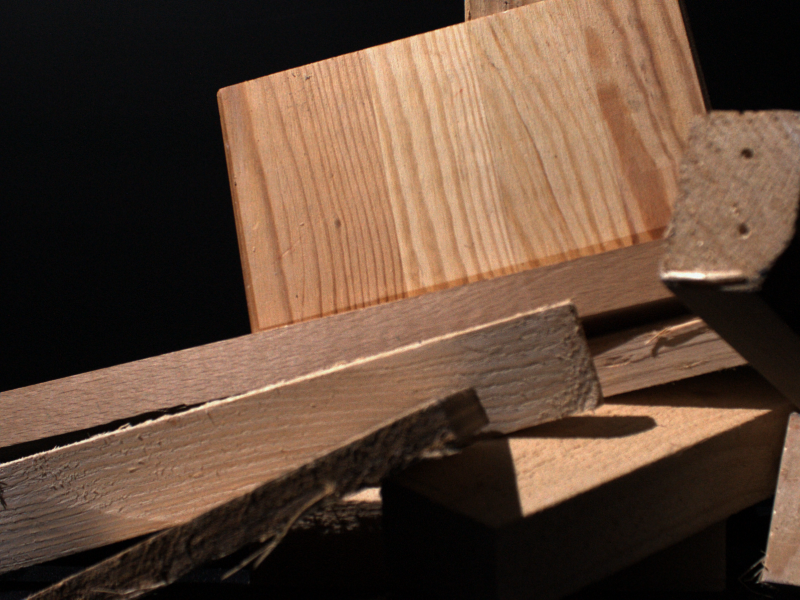
\includegraphics[width=\textwidth]{img/dtu_example_2.png}
	\end{subfigure}
	\par\medskip
	\begin{subfigure}{0.49\textwidth}
		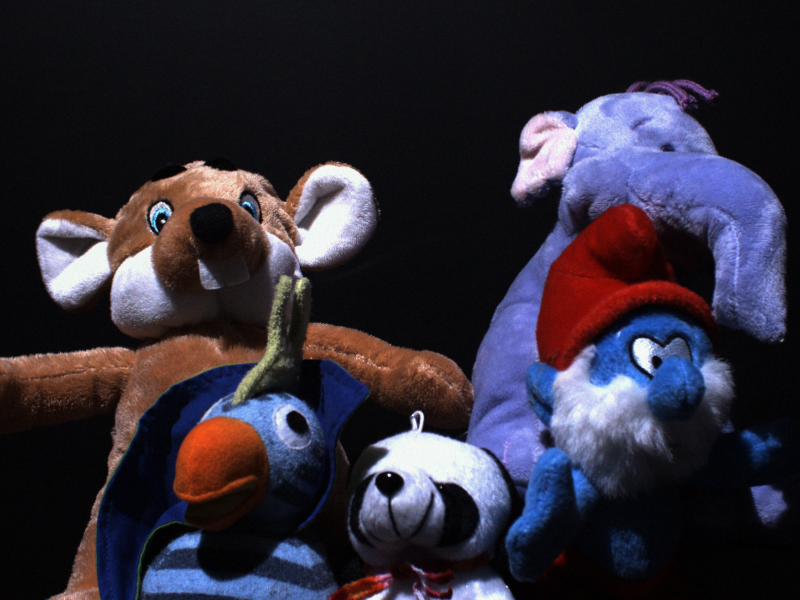
\includegraphics[width=\textwidth]{img/dtu_example_3.png}
	\end{subfigure}
	\hfill
	\begin{subfigure}{0.49\textwidth}
		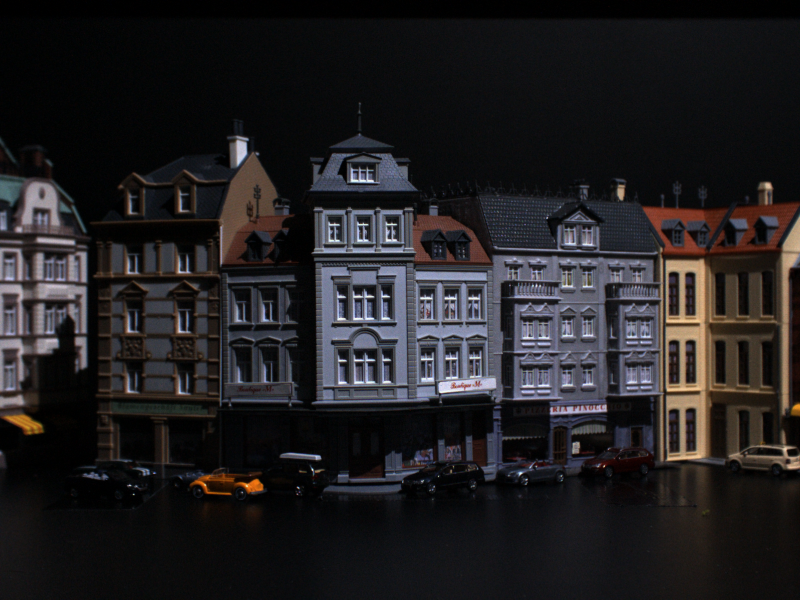
\includegraphics[width=\textwidth]{img/dtu_example_4.png}
	\end{subfigure}
	\caption{Example scenes from the DTU dataset}
	\label{fig:dtu_examples}
%
\vspace{1cm}
%
	\centering
	\begin{tabular}{l l r}
		\toprule
		Class & Scene numbers & Total \\
		\midrule
		House					& 1, 4, 8, 31, 32, 49, 50, 55				& 8 \\
		Books					& 2, 11, 20, 21								& 4 \\
		Fabric					& 5, 6, 45, 46, 47, 48						& 6 \\
		Greens					& 23, 24, 25, 26, 27, 51, 52, 53, 54, 56	& 10 \\
		Beer  					& 15, 16									& 2 \\
		Teddy Bears 			& 9, 10, 43, 44								& 4 \\
		Building Materials 		& 33, 34, 35, 36, 37						& 5 \\
		Decorative Items (Art) 	& 38, 39, 40, 41, 42						& 5 \\
		Groceries 				& 12, 28, 29, 30							& 4 \\
		Twigs and Leaves 		& 17, 57, 58, 59, 60 						& 5 \\
		\bottomrule
	\end{tabular}
	\caption{Scene object classifications from \cite[Table 1]{aanaes2010ground}}
	\label{tbl:dtu_scene_classifications}
\end{figure}

The camera is positioned around each scene using an industrial robot arm, which has automatically captured each scene from 119 positions. These positions are defined from a fixed frontal view varying the viewpoint $\theta$ in three arcs at different distance $d$ to the scene. Arc 1 has $d = \SI{0.5}{\meter}$ to the scene and $\theta$ spans $\SI{\pm40}{\degree}$, arc 2 has $d = \SI{0.65}{\meter}$ and $\theta$ spans $\SI{\pm25}{\degree}$, and arc 3 has $d = \SI{0.8}{\meter}$ and $\theta$ spans $\SI{\pm20}{\degree}$. Furthermore a linear path is captured by moving the camera away from the scene, which corresponds to zooming or scaling the scene. This is done at $\theta = \SI{0}{\degree}$ and $d$ spans $[\SI{0.5}{\meter};\SI{0.8}{\meter} ]$. At each of the 119 camera positions 19 individual images $I_i$ are taken with each of the LED lights $i,~\text{for}~i = 1,\hdots,19$ turned on. Using the given camera positions we get four camera paths: three arc paths and one linear path. \Cref{fig:dtu_overview} shows an overview of the four camera paths just described. When computing the performance across the paths we wish to solve the image correspondence problem for matching each image in each path with the \emph{keyframe} image (middle position on arc 1), since this gives us the performance when varying the viewing angle and scale in a structured manner.
%
\begin{figure}[p]
	\centering
	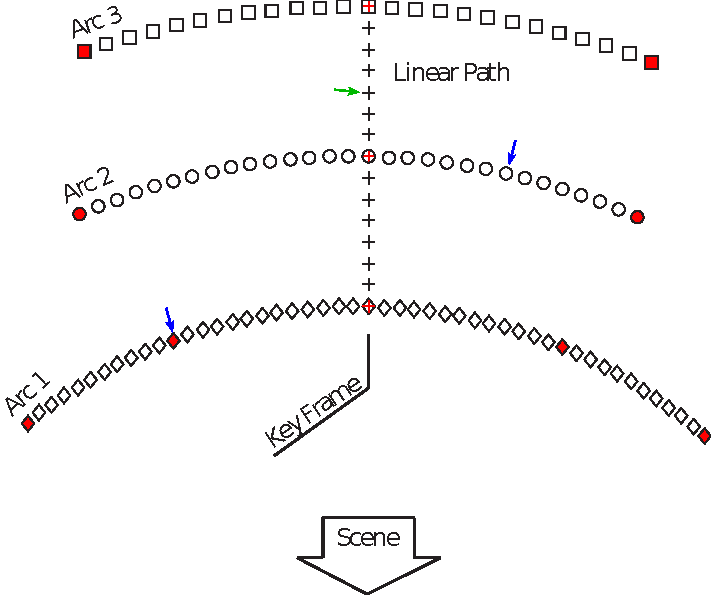
\includegraphics[width=0.9\textwidth]{img/CameraPosbOwn.pdf}
	\caption{Overview of camera positions and paths in the DTU dataset. The red positions mark training camera positions, the arrows mark camera positions of the light path experiments where only the ones marked with blue are used for training. Reconstructed and improved illustration from \citet[Figure 3, pp. 3]{aanaes2010recall}.}
	\label{fig:dtu_overview}
%\end{figure}
%\begin{figure}[tb]
	\vspace{1cm}
	\centering
	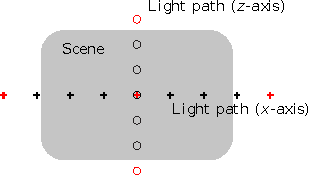
\includegraphics[width=0.7\textwidth]{img/dtu_light_overview.pdf}
	\caption{Light positions of the x- and z-axis light paths. Training light light positions marked with red. Reproduced and improved figure from \citet[Fig. 1, pp. 644]{larsen2012in}.}
	\label{fig:dtu_light_overview}
\end{figure}
%
The choice of capturing the scenes with individual LED lights created images with a high amount of cast shadows. \citet{larsen2012jet} created a set\footnote{dataset available at \url{http://roboimagedata.imm.dtu.dk/data/condensed.tar.gz}} of artificial diffuse and light paths from the individual LED images which we now briefly explain. The artificial diffuse light images are created from the individual lightings in order to only evaluate the performance of our descriptor under viewpoint changes and to get more natural images. These diffuse images are created by averaging over the individual light images for each camera position:
\begin{align}
	I_{\text{diffuse}} = \frac{1}{19} \sum_{i = 1}^{19} I_{i}
\end{align}
Since the dataset consists of individual LED images, one is able to construct images simulating two light source paths going from right to left and back to front respectively.
Given a light position ${\boldsymbol{x}}$ in the spatial domain of the LED positions, the image $I_{\boldsymbol{x}}$ is constructed by weighting each LED image by the Gaussian of the distance to ${\boldsymbol{x}}$:
\begin{align}
	I_{x} = \sum_{i = 1}^{19} G(\boldsymbol{x} - \boldsymbol{x}_i,\sigma) I_{i}
\end{align}
\Cref{fig:dtu_light_overview} shows the selected light positions. In order to get a somewhat general measurement for the robustness against light variations there are light paths generated for the following four image positions: 12 (arc 1), 25 (arc 1), 60 (linear path), and 87 (arc 2).
See \citet{aanaes2010recall,aanaes2010ground} for more information about the dataset and the generated light paths.

\Cref{fig:light_example} show 6 of the different light images for scene 4 at camera position 60. \Cref{fig:light_example_02,fig:light_example_17,fig:light_example_08} show the images taken with individual LED lighting (numbers 2, 17, and 8 respectively), and \Cref{fig:light_example_00} shows the diffuse light image. We here notice the significant difference in cast shadows using the three LEDs individually compared to the diffuse light image. The diffuse light image is however quite dark compared to the LED 8 light image, which could potentially cause problems in some scenes generating too few interest points. Such an issue could however be handled by adapting detection thresholds or by using histogram stretching/equalization.
\Cref{fig:light_example_28,fig:light_example_20} show the left- and rightmost positions of the X light path. By comparing these to their LED counterparts (\subref{fig:light_example_02} and \subref{fig:light_example_17} respectively) we see that the cast shadows are less significant therefore looking more natural.
\Cref{fig:viewpoint_example} shows 3 different camera positions for scene 4 including the keyframe (position 25).
%
\begin{figure}[tb]
	\centering
	\begin{subfigure}[t]{0.32\textwidth}
		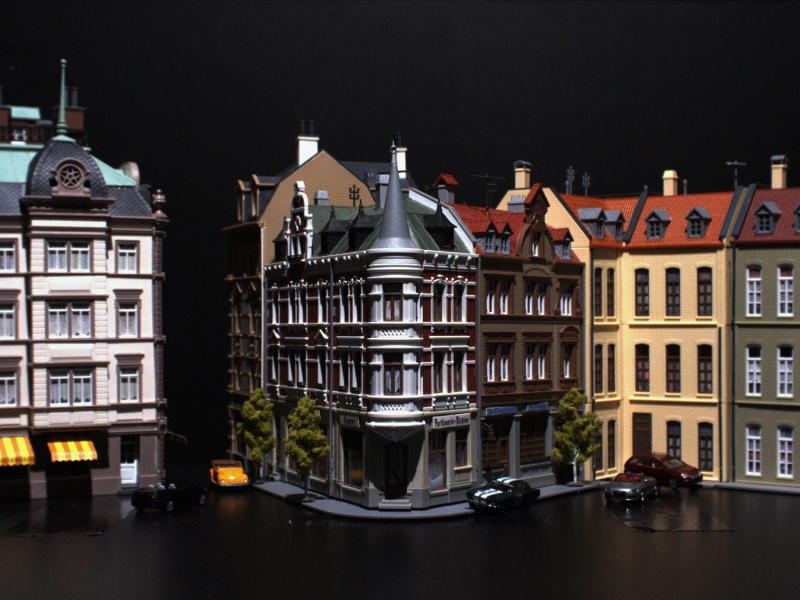
\includegraphics[width=\textwidth]{img/scene_04_img60_08.png}
		\caption{LED 8 light}
		\label{fig:light_example_08}
	\end{subfigure}
	\begin{subfigure}[t]{0.32\textwidth}
		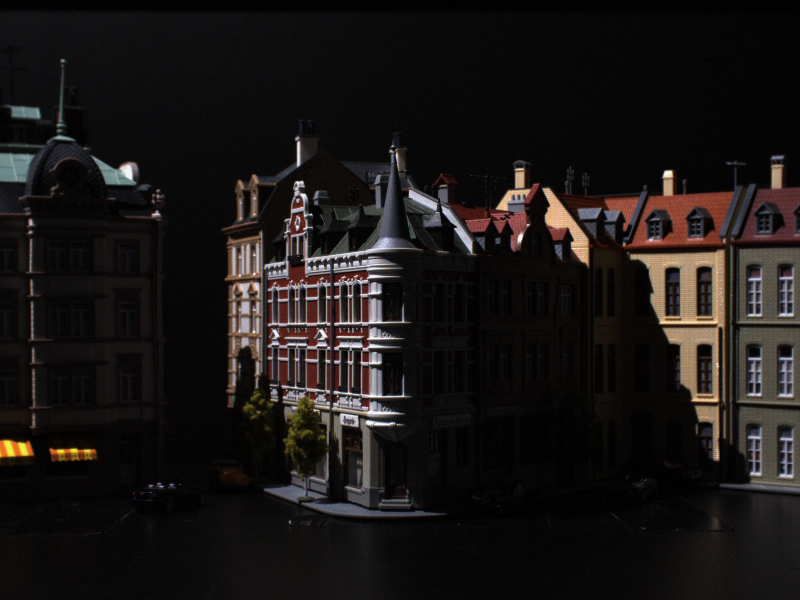
\includegraphics[width=\textwidth]{img/scene_04_img60_02.png}
		\caption{LED 2 light}
		\label{fig:light_example_02}
	\end{subfigure}
	\begin{subfigure}[t]{0.32\textwidth}
		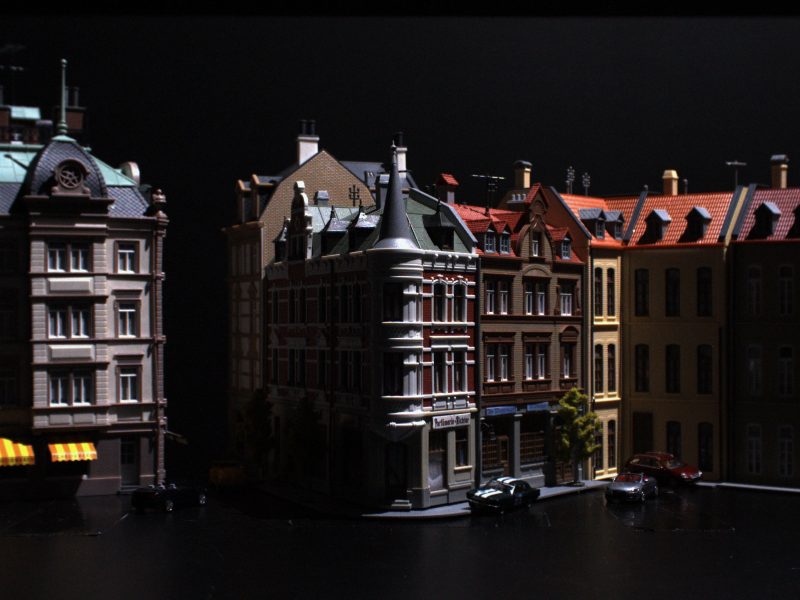
\includegraphics[width=\textwidth]{img/scene_04_img60_17.png}
		\caption{LED 17 light}
		\label{fig:light_example_17}
	\end{subfigure}
	\begin{subfigure}[t]{0.32\textwidth}
		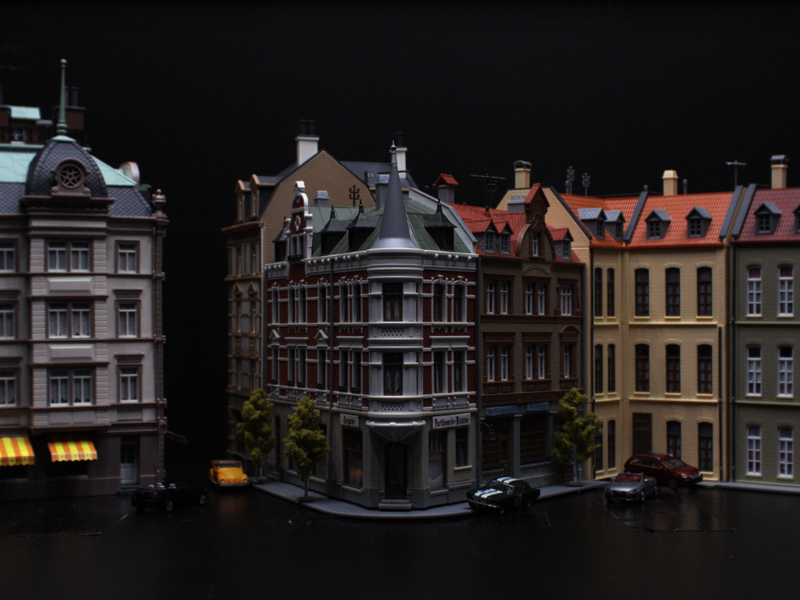
\includegraphics[width=\textwidth]{img/scene_04_img60_00.png}
		\caption{Diffuse light}
		\label{fig:light_example_00}
	\end{subfigure}
	\begin{subfigure}[t]{0.32\textwidth}
		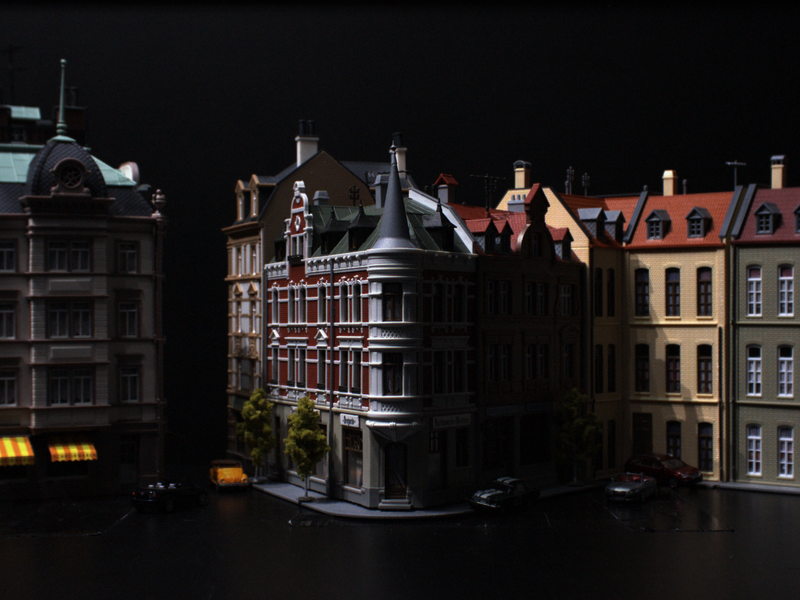
\includegraphics[width=\textwidth]{img/scene_04_img60_28.png}
		\caption{Leftmost position of X light path}
		\label{fig:light_example_28}
	\end{subfigure}
	\begin{subfigure}[t]{0.32\textwidth}
		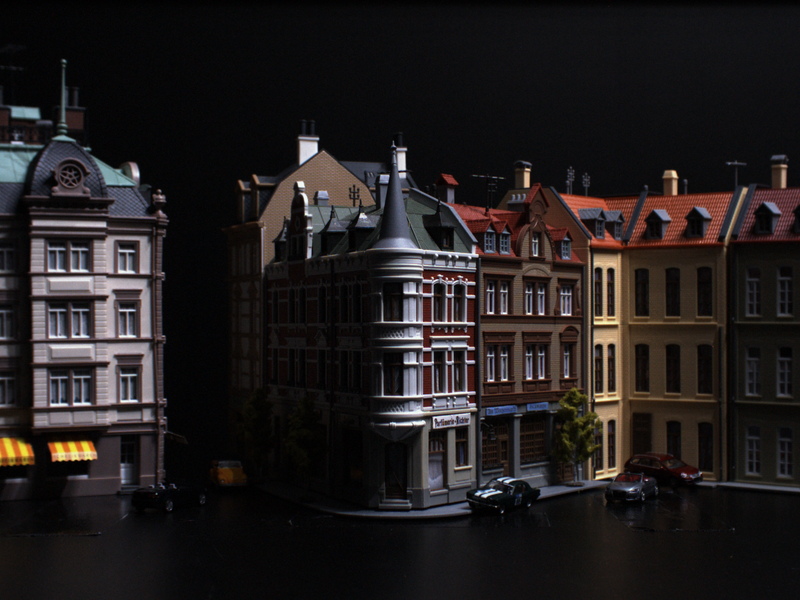
\includegraphics[width=\textwidth]{img/scene_04_img60_20.png}
		\caption{Rightmost position of X light path}
		\label{fig:light_example_20}
	\end{subfigure}
	\caption{Examples of light images in scene 4 at camera position 60.}
	\label{fig:light_example}
\end{figure}
%
\begin{figure}[tb]
	\centering
	\begin{subfigure}[t]{0.32\textwidth}
		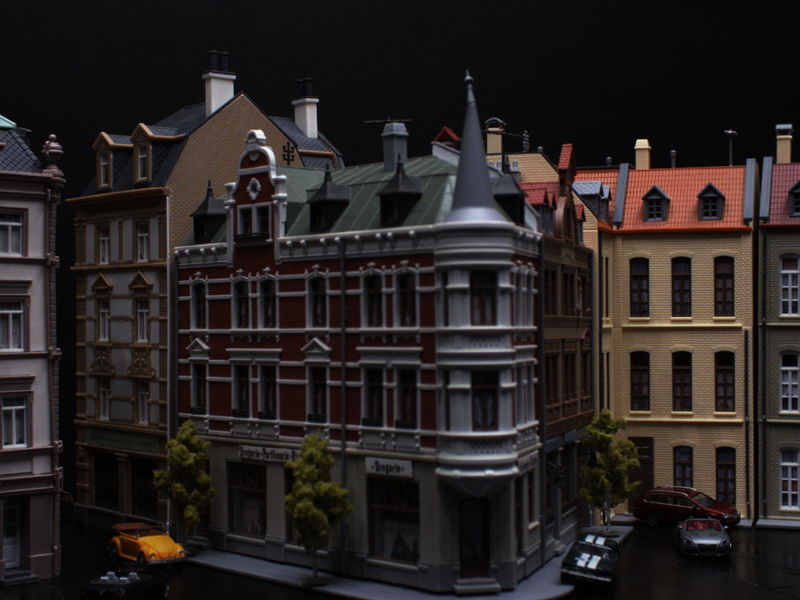
\includegraphics[width=\textwidth]{img/scene_04_img12_00.png}
		\caption{Camera position 12 (arc 1)}
		\label{fig:viewpoint_example_left}
	\end{subfigure}
	\begin{subfigure}[t]{0.32\textwidth}
		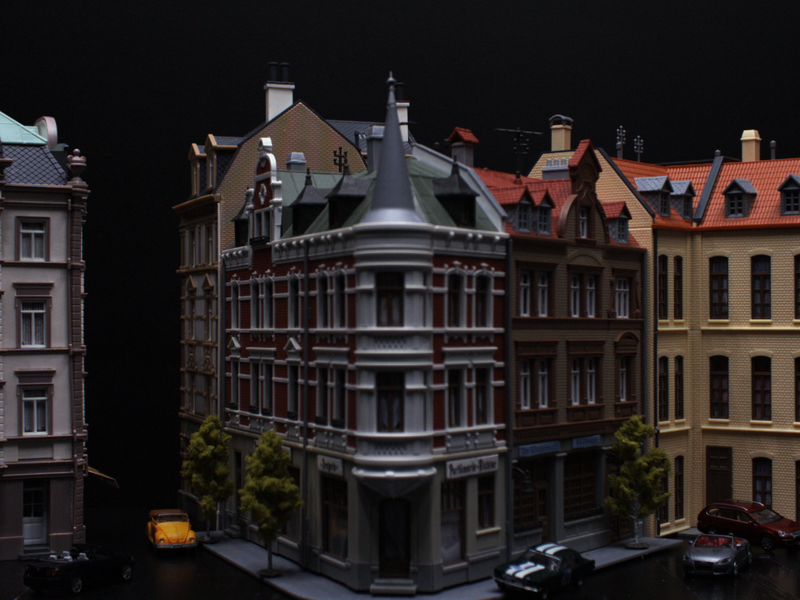
\includegraphics[width=\textwidth]{img/scene_04_img25_00.png}
		\caption{Camera position 25 (keyframe)}
		\label{fig:viewpoint_example_keyframe}
	\end{subfigure}
	\begin{subfigure}[t]{0.32\textwidth}
		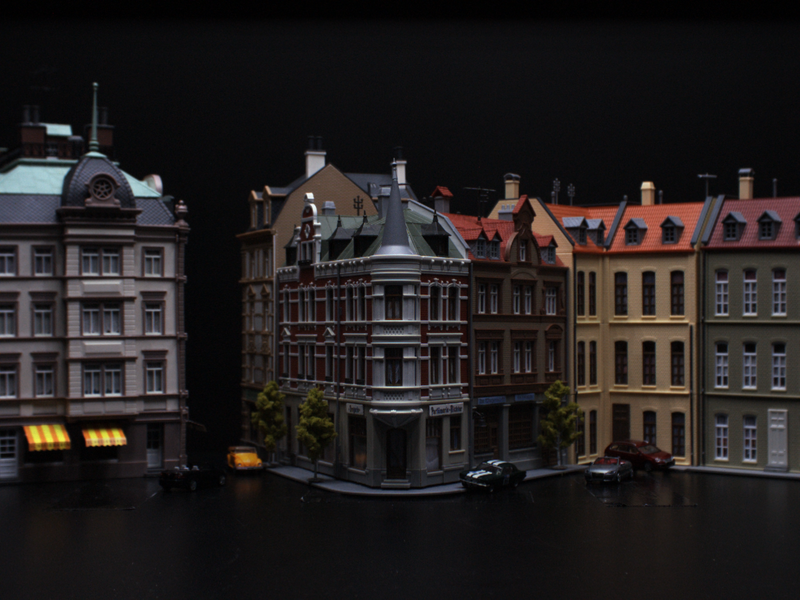
\includegraphics[width=\textwidth]{img/scene_04_img64_00.png}
		\caption{Camera position 64 (linear path)}
		\label{fig:viewpoint_example_scale}
	\end{subfigure}
	\caption{Examples of various camera positions of scene 4 using diffuse light.}
	\label{fig:viewpoint_example}
\end{figure}
%
\subsection{Evaluation}
In order to be able to classify matches between two images $A$ and $B$ as true or false, we need an evaluation method. In other words we need to compute/generate the match ground truth. The DTU dataset has been scanned using \emph{structured light} generating point clouds for the surfaces in each image. Using these points and the known camera positions for each image we are able to check if a matching of two points from $A$ and $B$ indeed correspond to 3D points close enough to one another to be true. \citet{aanaes2010recall} defined three evaluation criteria, of which we will be using the two first: Epipolar and surface geometry. We first define the property of being 3D reconstructable: an image point is said to be 3D reconstructable if there exists a point from the surface point cloud within a 10 pixel window in the image plane. This corresponds to a pixel within approximately 6 mm in the surface point cloud. Sometimes a matching is made for a point which is not 3D reconstructable. In this case no ground truth can be calculated, and the matching is ignored in the performance evaluation. The following two criteria (illustrated in \Cref{fig:icEvalGT}) determine the matching correspondence ground truth of the two points:
\begin{itemize}
	\item \textbf{Epipolar geometry consistency:} Given a point in the first image, the point in the second image should be within a 2.5 pixel orthogonal distance to the epipolar line of the first point as illustrated in \Cref{fig:icEval1GT}.
	\item \textbf{Surface geometry consistency:} The points need to be 3D reconstructible and they need to be within 3 mm of each other in the surface point cloud as illustrated in \Cref{fig:icEval2GT}.
\end{itemize}
The evaluation described in this section has been implemented by \citet{aanaes2010recall}. In this thesis we have used and improved their implementation for our evaluation of descriptor performance.

\mycomment[MSN]{Should we refer to \cite{larsen2012in}?}

\begin{figure}[tb]
	\centering
	\begin{subfigure}[t]{0.8\textwidth}
		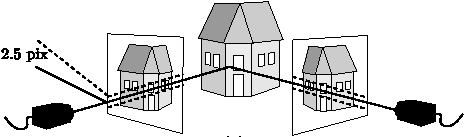
\includegraphics[width=\textwidth]{img/icEval1GT.pdf}
		\caption{Epipolar geometry consistency. Corresponding points should have an orthogonal distance to each others epipolar lines of maximum 2.5 pixel.}
		\label{fig:icEval1GT}
	\end{subfigure}
	\begin{subfigure}[t]{0.8\textwidth}
		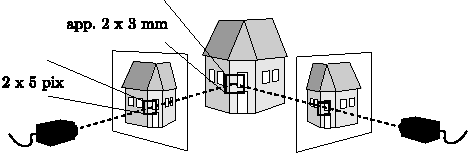
\includegraphics[width=\textwidth]{img/icEval2GT.pdf}
		\caption{Surface geometry consistency. Corresponding descriptors should be 3D reconstructable and be within 3 mm of each other in the surface point cloud.}
		\label{fig:icEval2GT}
	\end{subfigure}
	\caption{Illustration of the two ground truth evaluation criteria. Figure reproduced from \cite[Figure 5 (a-b),pp. 4]{aanaes2010recall}}
	\label{fig:icEvalGT}
\end{figure}

%
\subsection{Pitfalls and deficiencies}
The DTU dataset is built to test the ability of computer vision systems to cope with viewpoint changes, scaling, light changes, and to a certain extent occlusions as well. Since all images are captured with the same camera tilt, no rotation of objects occurs and hence rotational invariance and robustness cannot be evaluated using this dataset.

\Cref{fig:dtu_problems} shows the problems we have found within the DTU dataset, which we will go through here.

The artificial diffuse light is, as mentioned in the previous section, created by combining images captured under individual LED lighting. This is not optimal as some of the images are visually suffering from the spatial layout of the LED lights. \Cref{fig:dtu_problems_diffuse} shows image 20 (arc 1) from set 2 of the dataset. The diffuse light problem is clearly visible in the cast shadows seen on the 1st and 3rd book in the stack of lying books. Ideally these shadows would form either a smoothed or a single hard shadow edge instead of a number of gradually fading hard edges.

The automatic capturing of images using a robot arm combined with the individual LED lighting has the side-effect of the robot arm casting shadows in some of the images. This is seen when using the 3rd LED light and having captured the scenes from the far left of arc 1. \Cref{fig:dtu_problems_robot} shows an example of a cast shadow originating from the robot arm. This is however only a problem with one of the 19 LED light images and hence the effect on the final test images is minimal.
%
\begin{figure}[tb]
	\centering
	\begin{subfigure}{0.49\textwidth}
		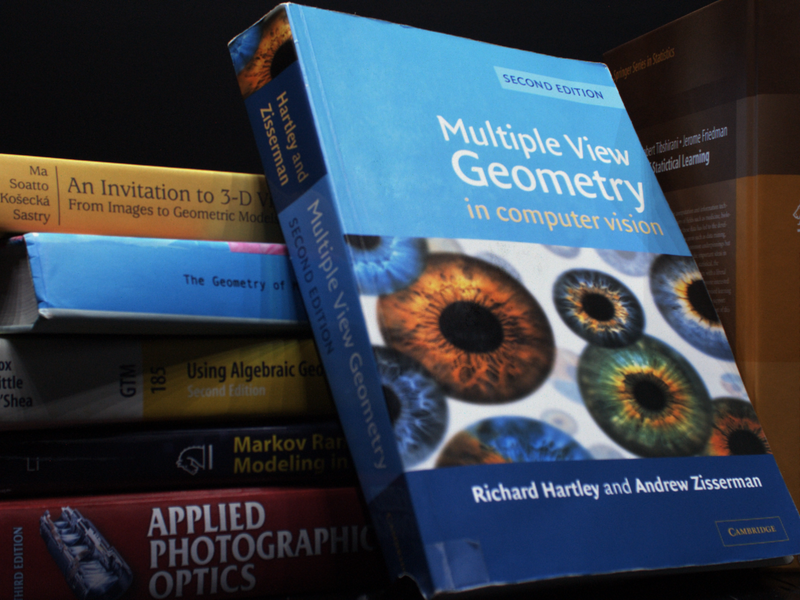
\includegraphics[width=\textwidth]{img/diffuse_light_problem.png}
		\caption{Diffuse lighting in set 2, image 20, with shadow artifacts}
		\label{fig:dtu_problems_diffuse}
	\end{subfigure}
	\begin{subfigure}{0.49\textwidth}
		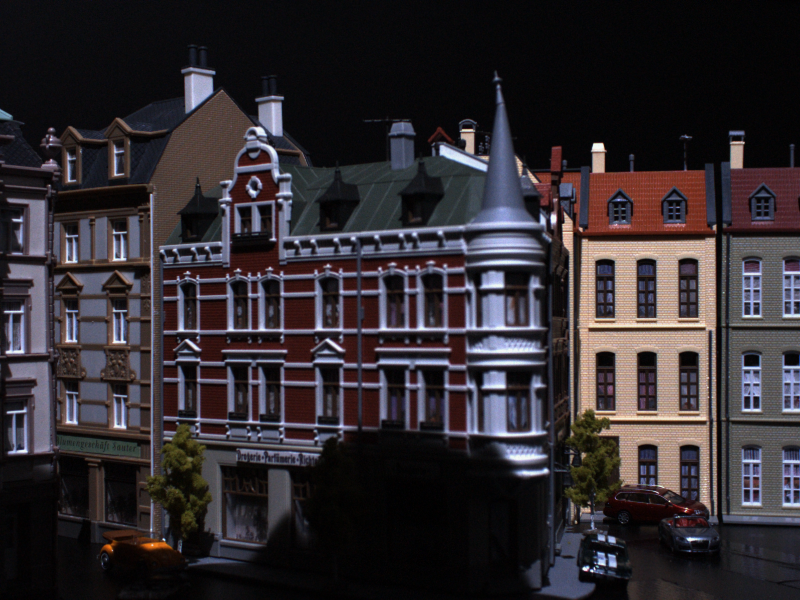
\includegraphics[width=\textwidth]{img/robot_arm_shadow.png}
		\caption{Robot arm shadow in set 4, image 7, LED light 3}
		\label{fig:dtu_problems_robot}
	\end{subfigure}
	\caption{Examples of problematic images in the DTU dataset}
	\label{fig:dtu_problems}
\end{figure}
%
\section{Experimental setup}
%
The DTU dataset is constructed using four different camera movement paths: Arc 1 through 3 and the linear path described in \Cref{sec:dtuDataset}. We therefore choose to perform one experiment for each of these paths, where we average across the different scenes for each camera position. These four experiments are all conducted using the diffuse light images. Furthermore we conduct two light experiments, where we move the light in the x- and z-axis respectively. For these experiments we both average across scenes and a fixed set of camera positions. In total we have six different experiments with perspective, scale and light transformations.

Since the DTU dataset is not split in a test and a train part, there is no pre-defined way of training and testing an algorithm on the dataset. \citet{larsen2012jet} used the Oxford Affine Covariance Region\footnote{\url{http://www.robots.ox.ac.uk/~vgg/research/affine}} dataset for manual parameter optimization of their Jet-based local image descriptors. This dataset is however very small and limited and hence we risk severe overfitting to the dataset if used for training. Instead we choose to split the DTU dataset with respect to the scenes into six parts for the purpose of (leave-one-out) cross-validation.

Testing is done on the full dataset, whereas we only perform training on a subset of the camera and light positions, since the dataset contains quite a large amount of images to be processed. \Cref{fig:dtu_overview} shows the camera positions of the dataset as described in \Cref{sec:dtuDataset}. In this illustration the training camera positions for the three arcs and the linear path are marked with red. The camera positions for the light experiments are marked with arrows, where only the ones marked with blue arrows are used for training. \Cref{fig:dtu_light_overview} shows the light positions for the light experiments. The red pluses and circles mark the x- and z-axis light path images used for training respectively.
%
\section{Example}
%
In this section we will continue the example from \Cref{sec:proposedDescriptorExample} by extending it to show the results of solving the image correspondence problem between the image of the example and the corresponding keyframe image from the DTU robot dataset.
\Cref{fig:imageCorrespondenceMatches} shows matches between the descriptors from the two images with score $s$ below threshold $t = 0.8$. The green and red lines indicate true and false positive classifications respectively. The images contain several similar beer cans and hence many of the false positive classifications are caused by patterns that are visible in multiple of the cans.

\Cref{fig:imageCorrespondenceCorrectMatch,fig:imageCorrespondenceIncorrectMatch} show two examples of a true positive match and a true negative match respectively. The green line shows a condition positive match and the red lines show condition negative matches. In \Cref{fig:imageCorrespondenceCorrectMatch} we see that there indeed is a correspondence between the best match of the two images with distance 0.083, and that our matching strategy results in a distance ratio (score) $s$ of 0.92. In \Cref{fig:imageCorrespondenceIncorrectMatch} we see that there is no match between the best matching descriptors of each image with distance 0.081. For this match $s$ is computed to 0.97. If we wanted to classify both matches correctly we should therefore set our threshold $t$ between 0.92 and 0.97. If we had used the distance as similarity measure we would not have been able to classify both correctly since the distance of the condition negative match is lower than the distance of the condition positive match.

When having computed the distance ratios of all matches, we are able to construct the ROC- and PR-curves giving us two measures of the performance of the descriptor matching. \Cref{fig:imageCorrespondenceCurves} shows the ROC-curve \subref{fig:imageCorrespondenceROC} and PR-curve \subref{fig:imageCorrespondencePR} as well as the area under the two curves. The match has a ROC AUC of 0.72 and PR AUC of 0.63. From the ROC plot wee see that the descriptor matching performs better than a random classification since the ROC-curve (blue line) lies above the curve of no predictive value (dashed line). This is likewise indicated by the ROC AUC which is above the random classification ROC AUC of 0.5.

%\newgeometry{left=2cm,right=2cm,top=3cm,bottom=3cm}
\begin{figure}[p]
	\centerline{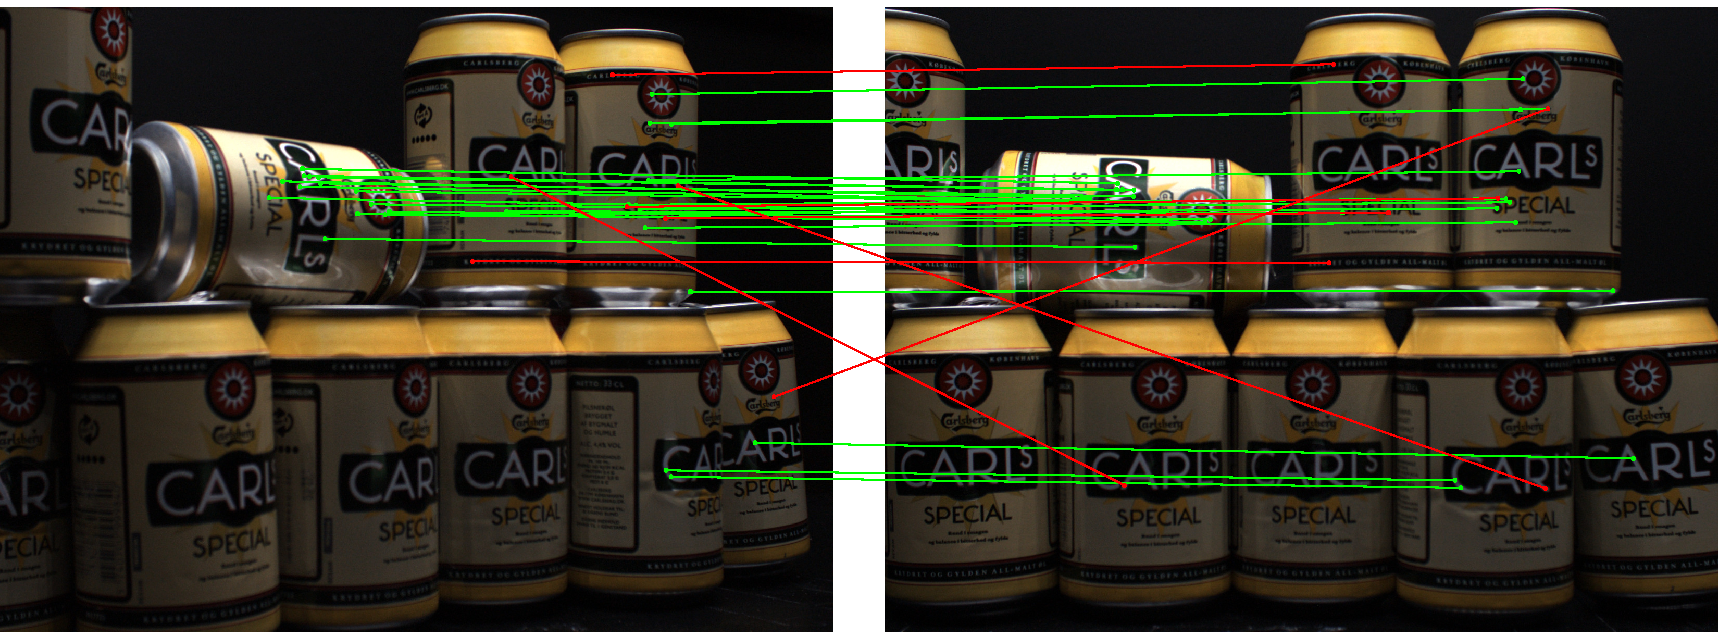
\includegraphics[width=1.1\textwidth]{img/imageCorrespondenceMatches.pdf}}
	\caption{Matches with score $s$ below threshold $t = 0.8$. Condition positive and negative matches are shown in green and red, respectively.}
	\label{fig:imageCorrespondenceMatches}
	\vspace{5mm}
	%
	\centerline{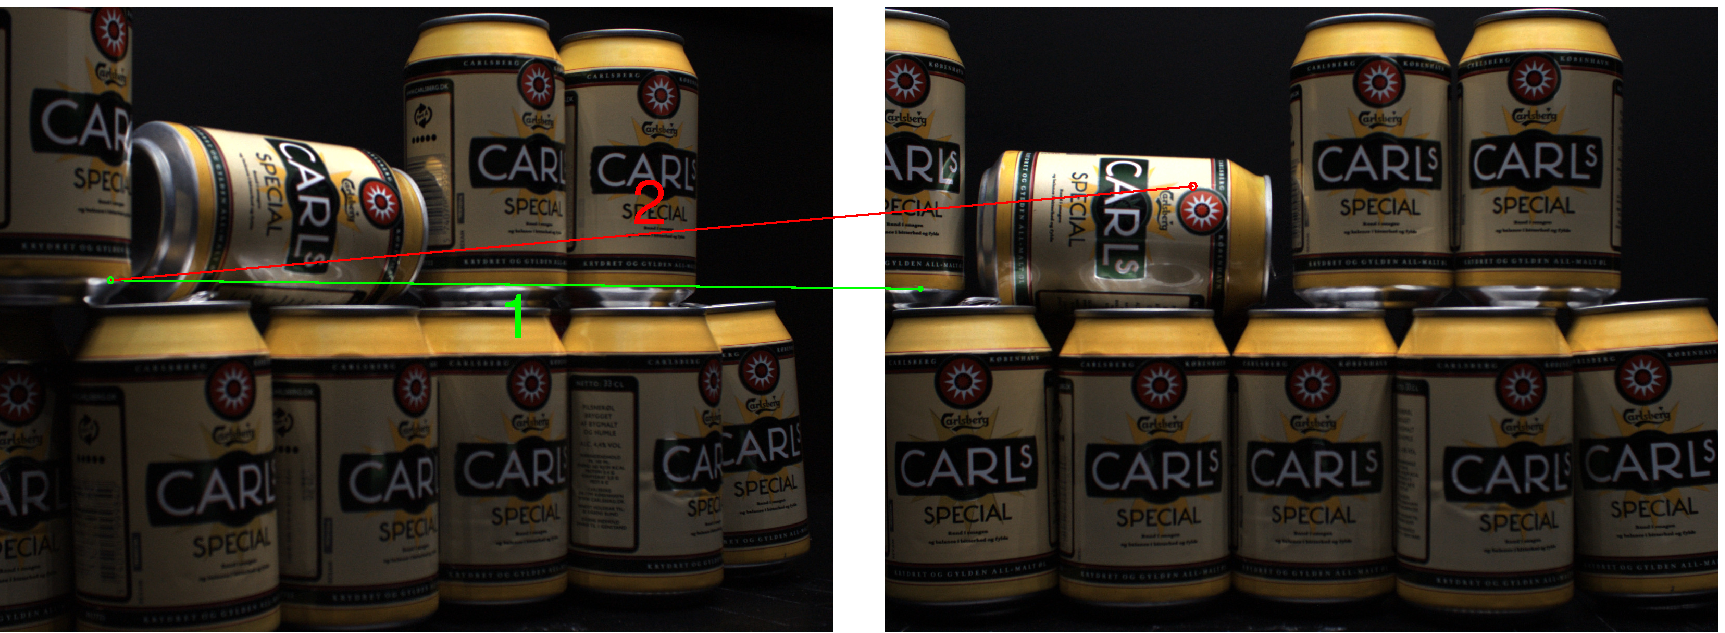
\includegraphics[width=1.1\textwidth]{img/imageCorrespondenceCorrectMatch.pdf}}
	\caption{Example of a condition positive match. First (1) and second (2) best matches have descriptor distances $0.076$ and $0.083$, respectively, resulting in a distance ratio of $0.92$.}
	\label{fig:imageCorrespondenceCorrectMatch}
	\vspace{5mm}
	%
	\centerline{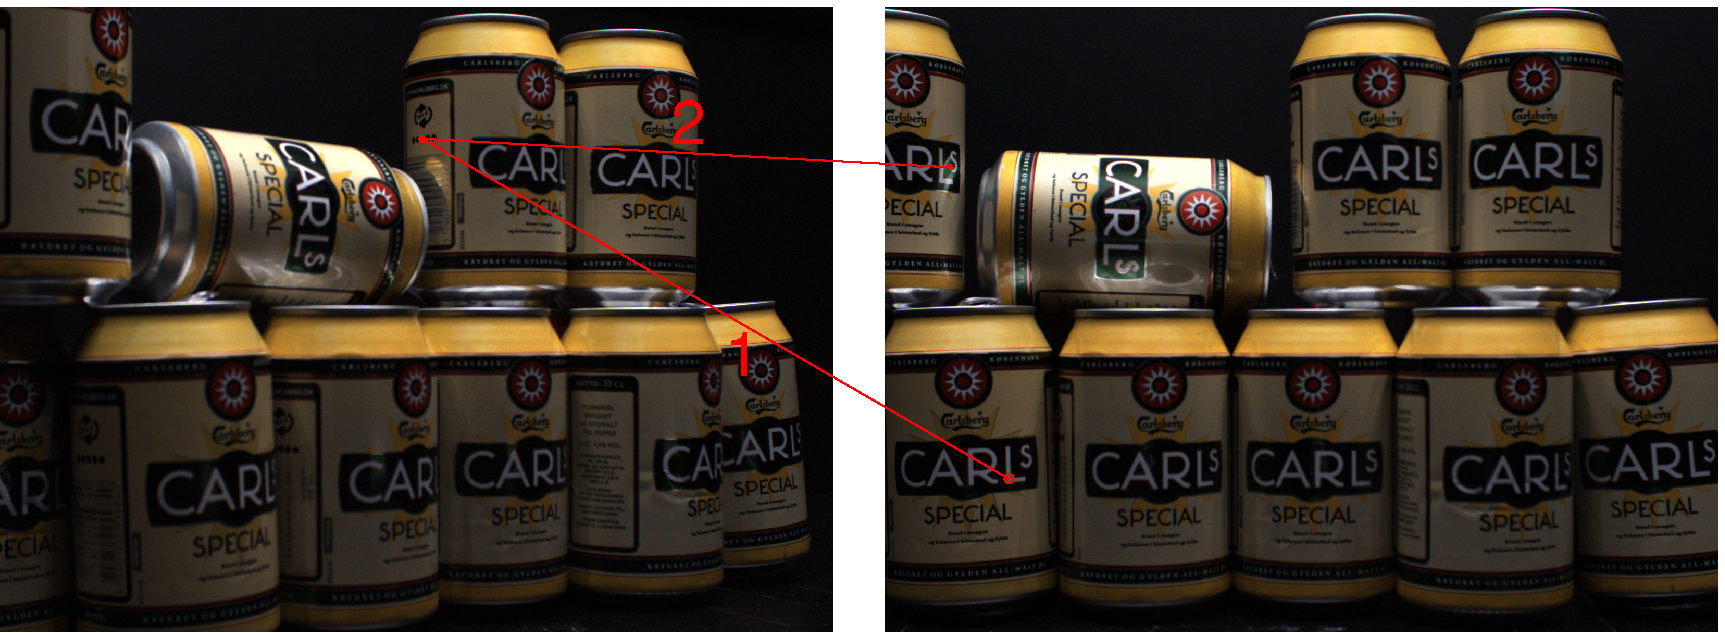
\includegraphics[width=1.1\textwidth]{img/imageCorrespondenceIncorrectMatch.pdf}}
	\caption{Example of an condition negative match. First (1) and second (2) best matches have descriptor distances $0.079$ and $0.081$, respectively, resulting in a distance ratio of $0.97$.}
	\label{fig:imageCorrespondenceIncorrectMatch}
\end{figure}
%\restoregeometry
%
\begin{figure}[tb]
	\centering
	\begin{subfigure}[t]{0.49\textwidth}
		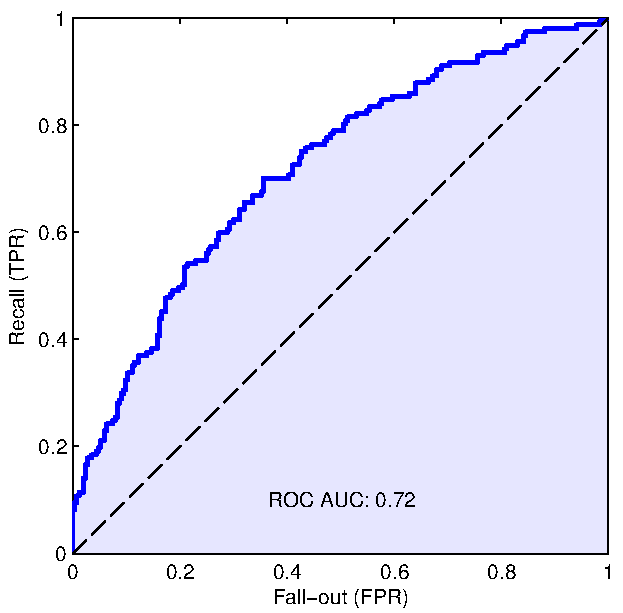
\includegraphics[width=\textwidth]{img/imageCorrespondenceROC.pdf}
		\caption{ROC-curve (blue line), curve of no predictive value attained by classifying randomly (dashed line), and area under the ROC-curve (light blue area)}
		\label{fig:imageCorrespondenceROC}
	\end{subfigure}
	\begin{subfigure}[t]{0.49\textwidth}
		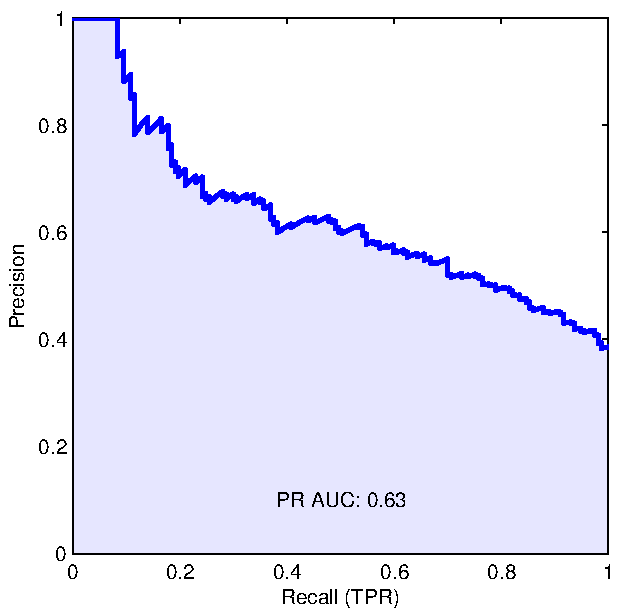
\includegraphics[width=\textwidth]{img/imageCorrespondencePR.pdf}
		\caption{PR-curve (blue line), area under the PR-curve (light blue area)}
		\label{fig:imageCorrespondencePR}
	\end{subfigure}
	\caption{Examples of evaluation measure curves}
	\label{fig:imageCorrespondenceCurves}
\end{figure}
%
\section{Parameter study}
\label{sec:icParameterStudy}
%
%Test: 6 fold cross validation.
%Tune on 5 folds, test on 1.
%
%Notes:
%
%1. Iterative minimization
%2. Computationally heavy, many parameters, hard to say something about the correlation of the parameters:
%3. Each sub-optimization:
%3a. Enum: One of the enumerated choices
%3b. Zoom: (2 iterations, initially large interval, then small zoomed in interval)
%4. 
%
%1. Problems with boosting the noise when using pixel normalization?
We wish to optimize the descriptor parameters listed in \Cref{sec:descriptorParameters} with the objective of maximizing average matching PR AUC. As mentioned in the experimental setup, we have split the DTU dataset into six parts to reduce overfitting by cross-validation. For each iteration we optimize parameters on five parts and test the optimized descriptor on the final part. This means we obtain six sets of parameters and a single PR AUC for each image, where the images are evaluated without optimizing across their respective scenes. To save time evaluating parameters, we scale the images to half size and convert them to grayscale. The testing is done on the full scale images converted to opponent colour space as mentioned in \Cref{sec:opponentColourSpace}.

Our actual parameter optimization is problematic because we need to optimize ten parameters at once, and each evaluation is computationally heavy. Our basic strategy is thus to cycle through each parameter and optimize it separately while fixing the other parameters. We do this a number of iterations with the hope of reaching convergence.
The risk of this strategy is getting stuck in local optima. To avoid this, recall that we have defined the parameters to reduce correlation: e.g. when bin count $n$ is increased, the width of the bins is automatically reduced to compensate. We also select certain correlated parameters to optimize together: grid type with grid size, as well as cell and bin kernels with their respective scales. Furthermore we optimize continuous parameters in two steps: first a coarse search and then a finer search around the best result.

The optimal parameters of our parameter study for our GO and SI descriptors are shown in \Cref{fig:ICparamsGo,fig:ICparamsSi} respectively.
From these results we see that most of the parameters are quite stable across the splits.

------------- NOTES ---------------
Generally: Parameters quite stable across splits. GO center scale $\rho$ a bit unstable.

GO - SI parameter comparison
Same grid size. Close to the same grid radius. Other parameters differ.

-----
Grid layout notes:
------
Grid radius big compared to SIFT.
Concentric and "normal": Very small difference
Centrals slightly better
Log polar generally worse than polar.
12x2 many angular cells compared to GLOH and DAISY
%
\begin{table}[p]
\centerline{
\begin{tabular}{ l c c c c c c c}
\toprule
{} & \multicolumn{6}{c}{Splits} \\
Parameter & 1 & 2 & 3 & 4 & 5 & 6 & chosen \\ \midrule
Grid type & PC & CPC & PC & PC & PC & PC & \textbf{PC} \\
Grid size & $12 \times 2$ & $12 \times 2$ & $12 \times 2$ & $12 \times 2$ & $12 \times 2$ & $12 \times 2$ & \textbf{$\mathbf{12 \times 2}$} \\
Grid radius $r$ & $13.5$ & $13.0$ & $13.5$ & $13.5$ & $13.5$ & $13.5$ & $\mathbf{13.5}$ \\
Center scale $\rho$ & $1.4$ & $1.9$ & $1.5$ & $1.4$ & $1.7$ & $1.5$ & $\mathbf{1.6}$ \\
Cell kernel & \textit{G} & \textit{G} & \textit{G} & \textit{G} & \textit{G} & \textit{G} & \textbf{\textit{G}} \\
Cell scale $\alpha$ & $0.8$ & $0.9$ & $0.8$ & $0.8$ & $0.8$ & $0.8$ & $\mathbf{0.8}$ \\
Bin count $n$ & $12$ & $12$ & $12$ & $14$ & $12$ & $14$ & $\mathbf{12}$ \\
Bin kernel & \textit{G} & \textit{G} & \textit{G} & \textit{G} & \textit{G} & \textit{G} & \textbf{\textit{G}} \\
Bin scale $\beta$ & $1.3$ & $1.3$ & $1.3$ & $1.3$ & $1.3$ & $1.3$ & $\mathbf{1.3}$ \\
Norm. scale $\eta$ & $1.6$ & $1.6$ & $1.6$ & $1.6$ & $1.6$ & $1.8$ & $\mathbf{1.6}$ \\
\bottomrule
\end{tabular}}
\caption{Parameter study optimal parameters from 6-fold cross validation of GO}
\label{fig:ICparamsGo}
%
\vspace{1cm}
%
\centerline{
\begin{tabular}{ l c c c c c c c}
\toprule
{} & \multicolumn{6}{c}{Splits} \\
Parameter & 1 & 2 & 3 & 4 & 5 & 6 & chosen \\ \midrule
Grid type & CPC & CPC & CPC & CPC & CPC & CPC & \textbf{CPC} \\
Grid size & $12 \times 2$ & $12 \times 2$ & $12 \times 2$ & $12 \times 2$ & $12 \times 2$ & $12 \times 2$ & \textbf{$\mathbf{12 \times 2}$} \\
Grid radius $r$ & $13.5$ & $14.0$ & $13.5$ & $14.0$ & $14.0$ & $14.0$ & $\mathbf{14.0}$ \\
Center scale $\rho$ & $1.9$ & $2.0$ & $2.0$ & $2.0$ & $2.0$ & $2.0$ & $\mathbf{2.0}$ \\
Cell kernel & \textit{G} & \textit{G} & \textit{G} & \textit{G} & \textit{G} & \textit{G} & \textbf{\textit{G}} \\
Cell scale $\alpha$ & $1.1$ & $1.0$ & $1.1$ & $1.0$ & $1.0$ & $1.0$ & $\mathbf{1.0}$ \\
Bin count $n$ & $8$ & $8$ & $8$ & $8$ & $8$ & $8$ & $\mathbf{8}$ \\
Bin kernel & \textit{G} & \textit{G} & \textit{G} & \textit{G} & \textit{G} & \textit{G} & \textbf{\textit{G}} \\
Bin scale $\beta$ & $2.0$ & $2.0$ & $2.0$ & $2.0$ & $2.0$ & $2.0$ & $\mathbf{2.0}$ \\
Norm. scale $\eta$ & $2.6$ & $2.8$ & $2.6$ & $2.6$ & $2.6$ & $2.6$ & $\mathbf{2.6}$ \\
\bottomrule
\end{tabular}}
\caption{Parameter study optimal parameters from 6-fold cross validation of SI}
\label{fig:ICparamsSi}
\end{table}
%
\begin{table}[tb]
\centering
\begin{tabular}{ c c c c c c c }
\toprule
Grid size & P & CP & PC & CPC & LP & CLP \\ \midrule
$6 \times 2$ & $0.756$ & $0.756$ & $0.759$ & $0.759$ & $0.700$ & $0.732$ \\ 
$8 \times 2$ & $0.767$ & $0.767$ & $0.770$ & $0.770$ & $0.759$ & $0.763$ \\ 
$10 \times 2$ & $0.772$ & $0.772$ & $0.776$ & $0.776$ & $0.769$ & $0.769$ \\ 
$12 \times 2$ & $0.775$ & $0.775$ & $\mathbf{0.779}$ & $0.779$ & $0.770$ & $0.767$ \\ 
$6 \times 3$ & $0.763$ & $0.764$ & $0.770$ & $0.770$ & - & - \\ 
$8 \times 3$ & $0.771$ & $0.771$ & $0.777$ & $0.777$ & - & - \\ 
$6 \times 4$ & $0.758$ & $0.759$ & $0.767$ & $0.767$ & - & - \\ 
\bottomrule
\end{tabular}
\caption{Grid layout parameter study for GO}
\label{tbl:dtuLayoutParametersGo}
\end{table}
%
\begin{table}[tb]
\centering
\begin{tabular}{ c c c c c c c }
\toprule
Grid size & P & CP & PC & CPC & LP & CLP \\ \midrule
$6 \times 2$ & $0.684$ & $0.685$ & $0.691$ & $0.692$ & $0.633$ & $0.664$ \\ 
$8 \times 2$ & $0.712$ & $0.713$ & $0.720$ & $0.721$ & $0.707$ & $0.712$ \\ 
$10 \times 2$ & $0.729$ & $0.731$ & $0.739$ & $0.739$ & $0.726$ & $0.727$ \\ 
$12 \times 2$ & $0.738$ & $0.739$ & $0.748$ & $\mathbf{0.749}$ & $0.732$ & $0.729$ \\ 
$6 \times 3$ & $0.711$ & $0.713$ & $0.717$ & $0.718$ & - & - \\ 
$8 \times 3$ & $0.731$ & $0.733$ & $0.736$ & $0.738$ & - & - \\ 
$6 \times 4$ & $0.706$ & $0.707$ & $0.721$ & $0.720$ & - & - \\
\bottomrule
\end{tabular}
\caption{Grid layout parameter study for SI}
\label{tbl:dtuLayoutParametersSi}
\end{table}
%
\begin{figure}[p]
\centering
	\centerline{\begin{subfigure}[t]{0.593\textwidth}
		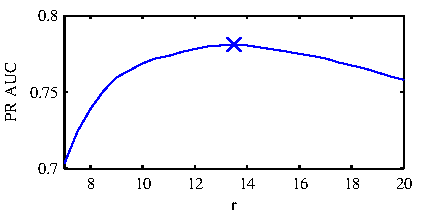
\includegraphics[width=\textwidth]{img/dtuParametersGo_gridRadius.pdf}
		\caption{Grid radius $r$}
		\label{fig:dtuParametersGo_gridRadius}
	\end{subfigure}
	\begin{subfigure}[t]{0.593\textwidth}
		\centering
		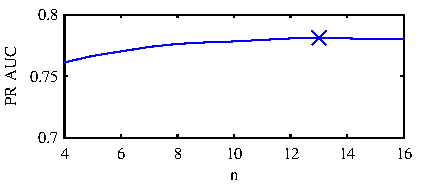
\includegraphics[width=\textwidth]{img/dtuParametersGo_binCount.pdf}
		\caption{Bin count $n$}
		\label{fig:dtuParametersGo_binCount}
	\end{subfigure}}
	\centerline{\begin{subfigure}[t]{0.593\textwidth}
		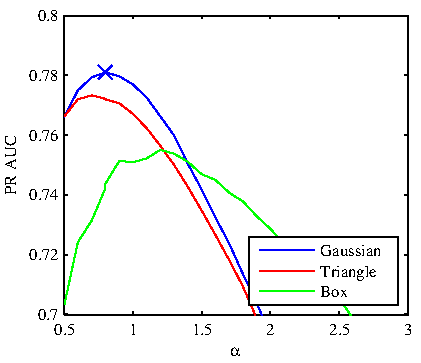
\includegraphics[width=\textwidth]{img/dtuParametersGo_cellSigmaAlt.pdf}
		\caption{Cell scale $\alpha$}
		\label{fig:dtuParametersGo_cellSigma}
		\vspace{2mm}
	\end{subfigure}
	\begin{subfigure}[t]{0.593\textwidth}
		\centering
		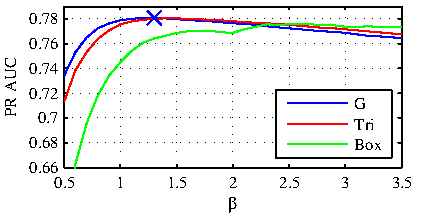
\includegraphics[width=\textwidth]{img/dtuParametersGo_binSigmaAlt.pdf}
		\caption{Bin scale $\beta$}
		\label{fig:dtuParametersGo_binSigma}
	\end{subfigure}}
	\centerline{\begin{subfigure}[t]{0.593\textwidth}
		\centering
		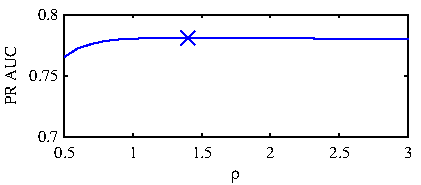
\includegraphics[width=\textwidth]{img/dtuParametersGo_centerSigma.pdf}
		\caption{Center scale $\rho$}
		\label{fig:dtuParametersGo_centerSigma}
		\vspace{2mm}
	\end{subfigure}
	\begin{subfigure}[t]{0.593\textwidth}
		\centering
		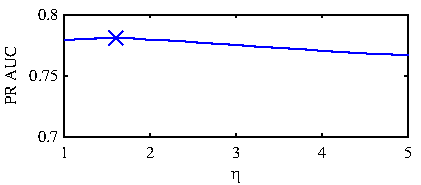
\includegraphics[width=\textwidth]{img/dtuParametersGo_normSigma.pdf}
		\caption{Normalization scale $\eta$}
		\label{fig:dtuParametersGo_normSigma}
		\vspace{2mm}
	\end{subfigure}}
	\caption{Parameter study results for GO.}
	\label{fig:dtuParametersGoAuc}
	\vspace{1cm}
	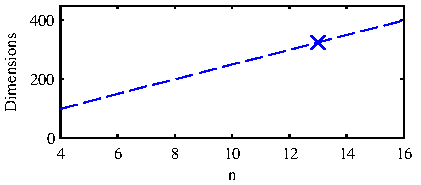
\includegraphics[width=0.593\textwidth]{img/dtuParametersGo_binCountDims.pdf}
	\caption{Dimensionality of GO based on bin count $n$}
	\label{fig:dtuParametersGoDims}
\end{figure}
%
\begin{figure}[p]
\centering
	\centerline{\begin{subfigure}[t]{0.593\textwidth}
		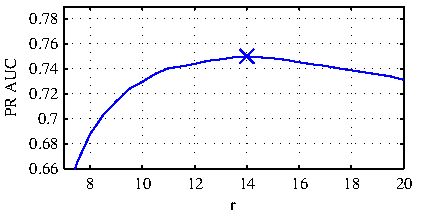
\includegraphics[width=\textwidth]{img/dtuParametersSi_gridRadius.pdf}
		\caption{Grid radius $r$}
		\label{fig:dtuParametersSi_gridRadius}
	\end{subfigure}
	\begin{subfigure}[t]{0.593\textwidth}
		\centering
		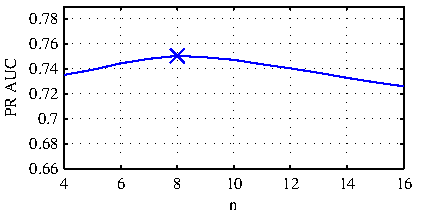
\includegraphics[width=\textwidth]{img/dtuParametersSi_binCount.pdf}
		\caption{Bin count $n$}
		\label{fig:dtuParametersSi_binCount}
	\end{subfigure}}
	\centerline{\begin{subfigure}[t]{0.593\textwidth}
		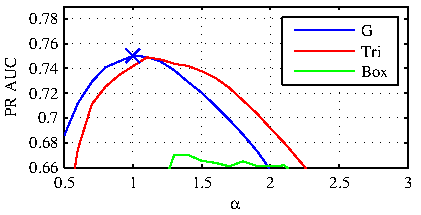
\includegraphics[width=\textwidth]{img/dtuParametersSi_cellSigmaAlt.pdf}
		\caption{Cell scale $\alpha$}
		\label{fig:dtuParametersSi_cellSigma}
		\vspace{2mm}
	\end{subfigure}
	\begin{subfigure}[t]{0.593\textwidth}
		\centering
		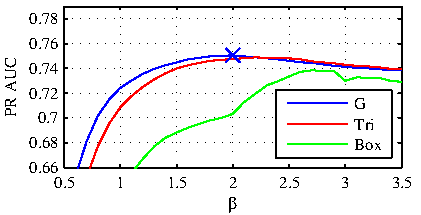
\includegraphics[width=\textwidth]{img/dtuParametersSi_binSigmaAlt.pdf}
		\caption{Bin scale $\beta$}
		\label{fig:dtuParametersSi_binSigma}
	\end{subfigure}}
	\centerline{\begin{subfigure}[t]{0.593\textwidth}
		\centering
		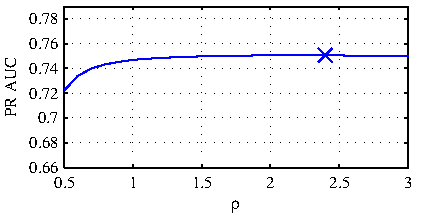
\includegraphics[width=\textwidth]{img/dtuParametersSi_centerSigma.pdf}
		\caption{Center scale $\rho$}
		\label{fig:dtuParametersSi_centerSigma}
		\vspace{2mm}
	\end{subfigure}
	\begin{subfigure}[t]{0.593\textwidth}
		\centering
		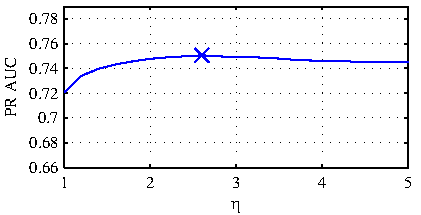
\includegraphics[width=\textwidth]{img/dtuParametersSi_normSigma.pdf}
		\caption{Normalization scale $\eta$}
		\label{fig:dtuParametersSi_normSigma}
		\vspace{2mm}
	\end{subfigure}}
	\caption{Parameter study results for SI.}
	\label{fig:dtuParametersSiAuc}
	\vspace{1cm}
	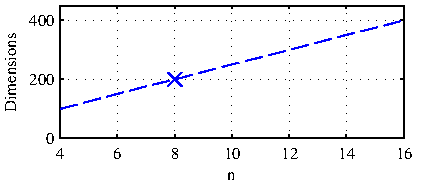
\includegraphics[width=0.593\textwidth]{img/dtuParametersSi_binCountDims.pdf}
	\caption{Dimensionality of SI based on bin count $n$}
	\label{fig:dtuParametersSiDims}
\end{figure}
%
%\begin{figure}[tb]
%	\centerline{\begin{subfigure}[t]{0.593\textwidth}
%		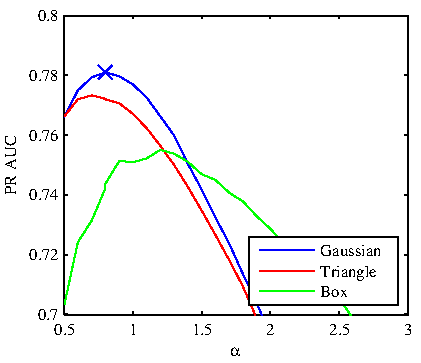
\includegraphics[width=\textwidth]{img/dtuParametersGo_cellSigmaAlt.pdf}
%		\caption{Cell scale $\alpha$}
%		\label{fig:dtuParametersGo_cellSigmaAlt}
%	\end{subfigure}
%	\begin{subfigure}[t]{0.593\textwidth}
%		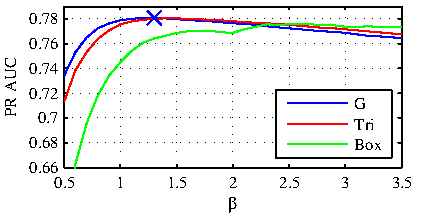
\includegraphics[width=\textwidth]{img/dtuParametersGo_binSigmaAlt.pdf}
%		\caption{Bin scale $\beta$}
%		\label{fig:dtuParametersGo_binSigmaAlt}
%	\end{subfigure}}
%	\caption{Alternative choices of cell and bin filters for GO.}
%	\label{fig:dtuParametersGoAlt}
%\end{figure}
%
We have also experimented with various other parts of our descriptor that are not listed as parameters. We report some of these results for our optimal GO descriptor on training data, which has a mean PR AUC of $0.781$: It is marginally better to normalize the final descriptors before searching for matches. Omitting this step reduces the AUC by $0.002$. Doubling the image resolution improves the AUC by $0.009$. Computing the descriptor on opponent colour channels improves the AUC by $0.014$. Omitting pixel normalization reduces the AUC by $0.023$. Omitting the center filter reduces the AUC by $0.002$.
%
\section{Results}
%
Having found the optimal parameters for each of the 6 splits in the previous section, we are now able to compute test results for each split and report the performance of our descriptors.
We have chosen to compare our descriptor performance against the SIFT descriptor since \citet{dahl2011finding} found the combination of DoG and SIFT to perform well. We are however using the opponent colour space for our descriptors, and since \citet{dahl2012interest} found Opponent SIFT (see \Cref{sec:SIFT}) to perform well against other SIFT variants, this is the descriptor we will test our performance against.

\Cref{fig:dtuResultsPR,fig:dtuResultsROC} show the mean PR and ROC AUC test results for the DTU dataset respectively. For both these measures the GO (red), SI (green), GO+SI (blue) and SIFT (dashed grey) results are shown. Recall from \Cref{sec:binaryClassificationMeasures} that an algorithm which optimizes PR AUC does not necessarily optimize ROC AUC. Despite this fact, the mean ROC AUCs for our descriptors compared to the SIFT ROC AUC are somewhat equal to the corresponding comparisons of mean PR AUCs. SI however has a slight advantage over GO and GO+SI when visually inspecting the mean ROC AUC figures. In \Cref{sec:performance_measures} we wrote that we gave the PR measure more importance than ROC, and hence The following comparison of performance between the descriptors is based on the PR AUC figures.

The first thing we notice when looking at all the graphs in \Cref{fig:dtuResultsPR} is, that our GO+SI descriptor is marginally better than GO on arc 1, but they have identical performance on the rest of the variations. Furthermore we notice that our SI descriptor is worse than GO and GO+SI.

When looking at the three arc graphs (\Cref{fig:dtuResultsPRarc1,fig:dtuResultsPRarc2,fig:dtuResultsPRarc3}), we see that GO and GO+SI performance drops less than SIFT when the camera is moved towards the outermost camera positions. The advantage over SIFT is however lower for arc 2 and 3 than arc 1. This difference could be caused by smaller perspective distortions at arc 2 and 3 since the distance to the camera is increased and the angular differences are smaller than for arc 1.
This hypothesis is likewise supported by the fact that all four descriptors have roughly equal performance over scale variations as shown in \Cref{fig:dtuResultsPRlinear}.

For light variations (\Cref{fig:dtuResultsPRxAxis,fig:dtuResultsPRzAxis}) our descriptors perform better than SIFT.

Having inspected the graphs for mean PR AUCs, we are now interested in knowing whether the descriptors are statistically significantly different. We therefore perform Welch's $t$-test as described in \Cref{sec:welchsTtest} on each of the path positions. The resulting 95\% confidence interval graphs on the difference between our GO+SI descriptor and SIFT are show in \Cref{fig:dtuResultsStats}. As we see from the graphs, the confidence intervals cross 0 for all positions apart from position 1, 7, 8, and 9 of the $x$-axis light path and position 16 of the $z$-axis light path. In other words we cannot conclude that GO+SI and SIFT are significantly different except on these outermost positions of the light paths.

Performing Welch's $t$-tests between other combinations of the GO, SI, GO+SI, and SIFT descriptors reveal that pairwise none of our descriptors are significantly different apart from GO, which is significantly better than SIFT on position 6 to 9 of the $x$-axis light path and position 16 of the $z$-axis light path. Furthermore we cannot conclude that SIFT is significantly better than any of our descriptors. Since the graphs for all these combinations are both space-consuming and not too informative once we have the above conclusions, we have chosen to omit them. \mycomment[MSN]{Should we include all the combination statistic figures in an appendix?}
%
\begin{table}[tb]
\centering
\begin{tabular}{ l c c c }
\toprule
Descriptor & Dimensions & PR AUC & ROC AUC \\ \midrule
GO & $900/1050$ & $0.850$ & $0.888$ \\ 
SI & $600$ & $0.839$ & $0.890$ \\ 
GO+SI & $1500/1650$ & $0.851$ & $0.889$ \\ 
SIFT & $384$ & $0.831$ & $0.880$ \\ 
\bottomrule
\end{tabular}
\caption{Average performance across all test images for the various descriptors. Note that GO has a variable number of dimensions because different bin counts were found optimal across the cross-validation splits.}
\label{tbl:dtuOverallResults}
\end{table}
%
\begin{figure}[tb]
	\centerline{
		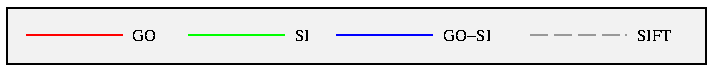
\includegraphics[width=1.2\textwidth]{img/dtuResults_opponent_legend_cropped.pdf}
	}	
	\centerline{
	\begin{subfigure}[t]{0.6242\textwidth}
		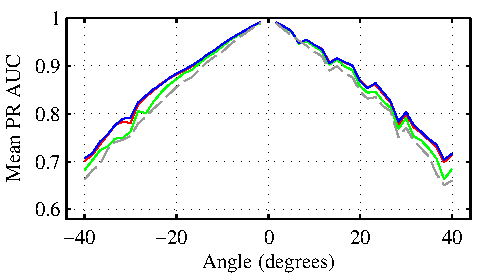
\includegraphics[width=\textwidth]{img/dtuResultsPR_opponent_1.pdf}
		\caption{Arc 1}
		\label{fig:dtuResultsPRarc1}
	\end{subfigure}
	\begin{subfigure}[t]{0.5618\textwidth}
		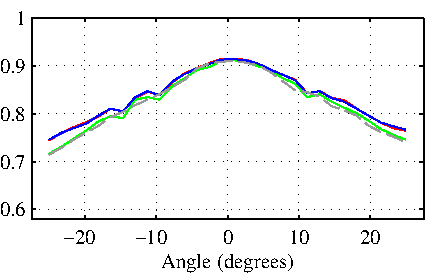
\includegraphics[width=\textwidth]{img/dtuResultsPR_opponent_2.pdf}
		\caption{Arc 2}
		\label{fig:dtuResultsPRarc2}
	\end{subfigure}
	}
	\centerline{
	\begin{subfigure}[t]{0.6242\textwidth}
		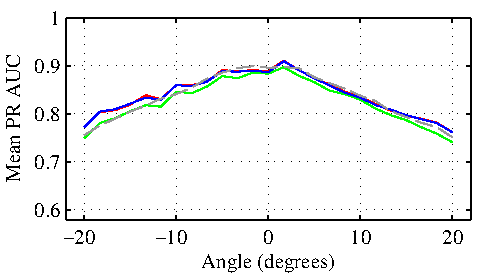
\includegraphics[width=\textwidth]{img/dtuResultsPR_opponent_3.pdf}
		\caption{Arc 3}
		\label{fig:dtuResultsPRarc3}
	\end{subfigure}
	\begin{subfigure}[t]{0.5618\textwidth}
		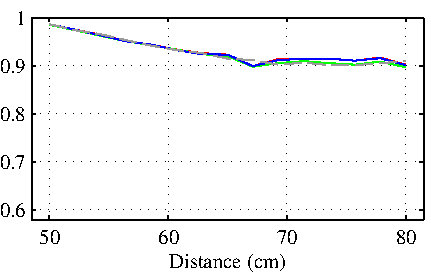
\includegraphics[width=\textwidth]{img/dtuResultsPR_opponent_4.pdf}
		\caption{Linear path}
		\label{fig:dtuResultsPRlinear}
	\end{subfigure}
	}
	\centerline{
	\begin{subfigure}[t]{0.6242\textwidth}
		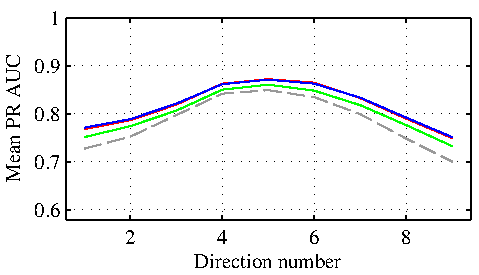
\includegraphics[width=\textwidth]{img/dtuResultsPR_opponent_5.pdf}
		\caption{Light path, $x$-axis}
		\label{fig:dtuResultsPRxAxis}
	\end{subfigure}
	\begin{subfigure}[t]{0.5618\textwidth}
		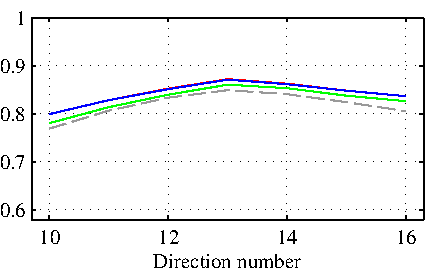
\includegraphics[width=\textwidth]{img/dtuResultsPR_opponent_6.pdf}
		\caption{Light path, $z$-axis}
		\label{fig:dtuResultsPRzAxis}
	\end{subfigure}
	}
	\caption{Mean PR AUC test results on the DTU dataset.}
	\label{fig:dtuResultsPR}
\end{figure}
%
\begin{figure}[tb]
	\centerline{
		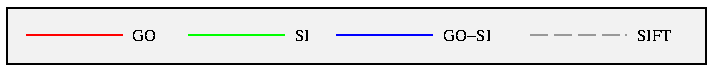
\includegraphics[width=1.2\textwidth]{img/dtuResults_opponent_legend_cropped.pdf}
	}	
	\centerline{
	\begin{subfigure}[t]{0.6242\textwidth}
		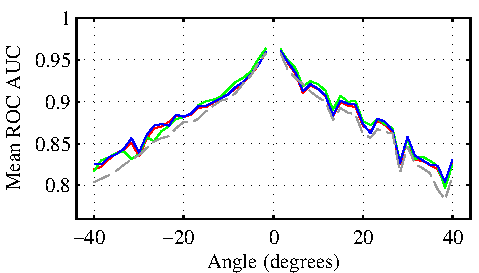
\includegraphics[width=\textwidth]{img/dtuResultsROC_opponent_1.pdf}
		\caption{Arc 1}
		\label{fig:dtuResultsROCarc1}
	\end{subfigure}
	\begin{subfigure}[t]{0.5618\textwidth}
		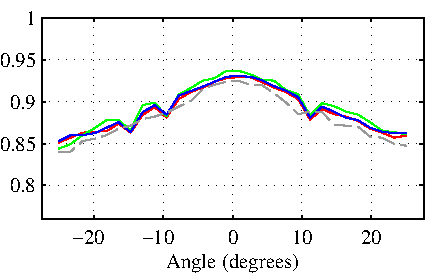
\includegraphics[width=\textwidth]{img/dtuResultsROC_opponent_2.pdf}
		\caption{Arc 2}
		\label{fig:dtuResultsROCarc2}
	\end{subfigure}
	}
	\centerline{
	\begin{subfigure}[t]{0.6242\textwidth}
		\includegraphics[width=\textwidth]{img/dtuResultsROC_opponent_3.pdf}
		\caption{Arc 3}
		\label{fig:dtuResultsROCarc3}
	\end{subfigure}
	\begin{subfigure}[t]{0.5618\textwidth}
		\includegraphics[width=\textwidth]{img/dtuResultsROC_opponent_4.pdf}
		\caption{Linear path}
		\label{fig:dtuResultsROClinear}
	\end{subfigure}
	}
	\centerline{
	\begin{subfigure}[t]{0.6242\textwidth}
		\includegraphics[width=\textwidth]{img/dtuResultsROC_opponent_5.pdf}
		\caption{Light path, $x$-axis}
		\label{fig:dtuResultsROCyAxis}
	\end{subfigure}
	\begin{subfigure}[t]{0.5618\textwidth}
		\includegraphics[width=\textwidth]{img/dtuResultsROC_opponent_6.pdf}
		\caption{Light path, $z$-axis}
		\label{fig:dtuResultsROCzAxis}
	\end{subfigure}
	}
	\caption{Mean ROC AUC test results on the DTU dataset paths.}
	\label{fig:dtuResultsROC}
\end{figure}
%
\begin{figure}[tb]
	\centerline{
	\begin{subfigure}[t]{0.6242\textwidth}
		\includegraphics[width=\textwidth]{img/dtuResultsStatsGoSi_Sift_1.pdf}
		\caption{Arc 1}
		\label{fig:dtuResultsStatsarc1}
	\end{subfigure}
	\begin{subfigure}[t]{0.5618\textwidth}
		\includegraphics[width=\textwidth]{img/dtuResultsStatsGoSi_Sift_2.pdf}
		\caption{Arc 2}
		\label{fig:dtuResultsStatsarc2}
	\end{subfigure}
	}
	\centerline{
	\begin{subfigure}[t]{0.6242\textwidth}
		\includegraphics[width=\textwidth]{img/dtuResultsStatsGoSi_Sift_3.pdf}
		\caption{Arc 3}
		\label{fig:dtuResultsStatsarc3}
	\end{subfigure}
	\begin{subfigure}[t]{0.5618\textwidth}
		\includegraphics[width=\textwidth]{img/dtuResultsStatsGoSi_Sift_4.pdf}
		\caption{Linear path}
		\label{fig:dtuResultsStatslinear}
	\end{subfigure}
	}
	\centerline{
	\begin{subfigure}[t]{0.6242\textwidth}
		\includegraphics[width=\textwidth]{img/dtuResultsStatsGoSi_Sift_5.pdf}
		\caption{Light path, $x$-axis}
		\label{fig:dtuResultsStatsxAxis}
	\end{subfigure}
	\begin{subfigure}[t]{0.5618\textwidth}
		\includegraphics[width=\textwidth]{img/dtuResultsStatsGoSi_Sift_6.pdf}
		\caption{Light path, $z$-axis}
		\label{fig:dtuResultsStatszAxis}
	\end{subfigure}
	}
	\caption{95\% confidence intervals on the PR AUC difference between our GO+SI descriptor and SIFT. A positive difference denotes that our GO+SI descriptor outperforms SIFT. If the confidence interval for a position contains zero, there is no significant difference in performance.}
	\label{fig:dtuResultsStats}
\end{figure}
%
%
\subbibliography
\end{document}
